\begin{frame}
	\frametitle{Obama the computer scientist}
	\begin{center}
		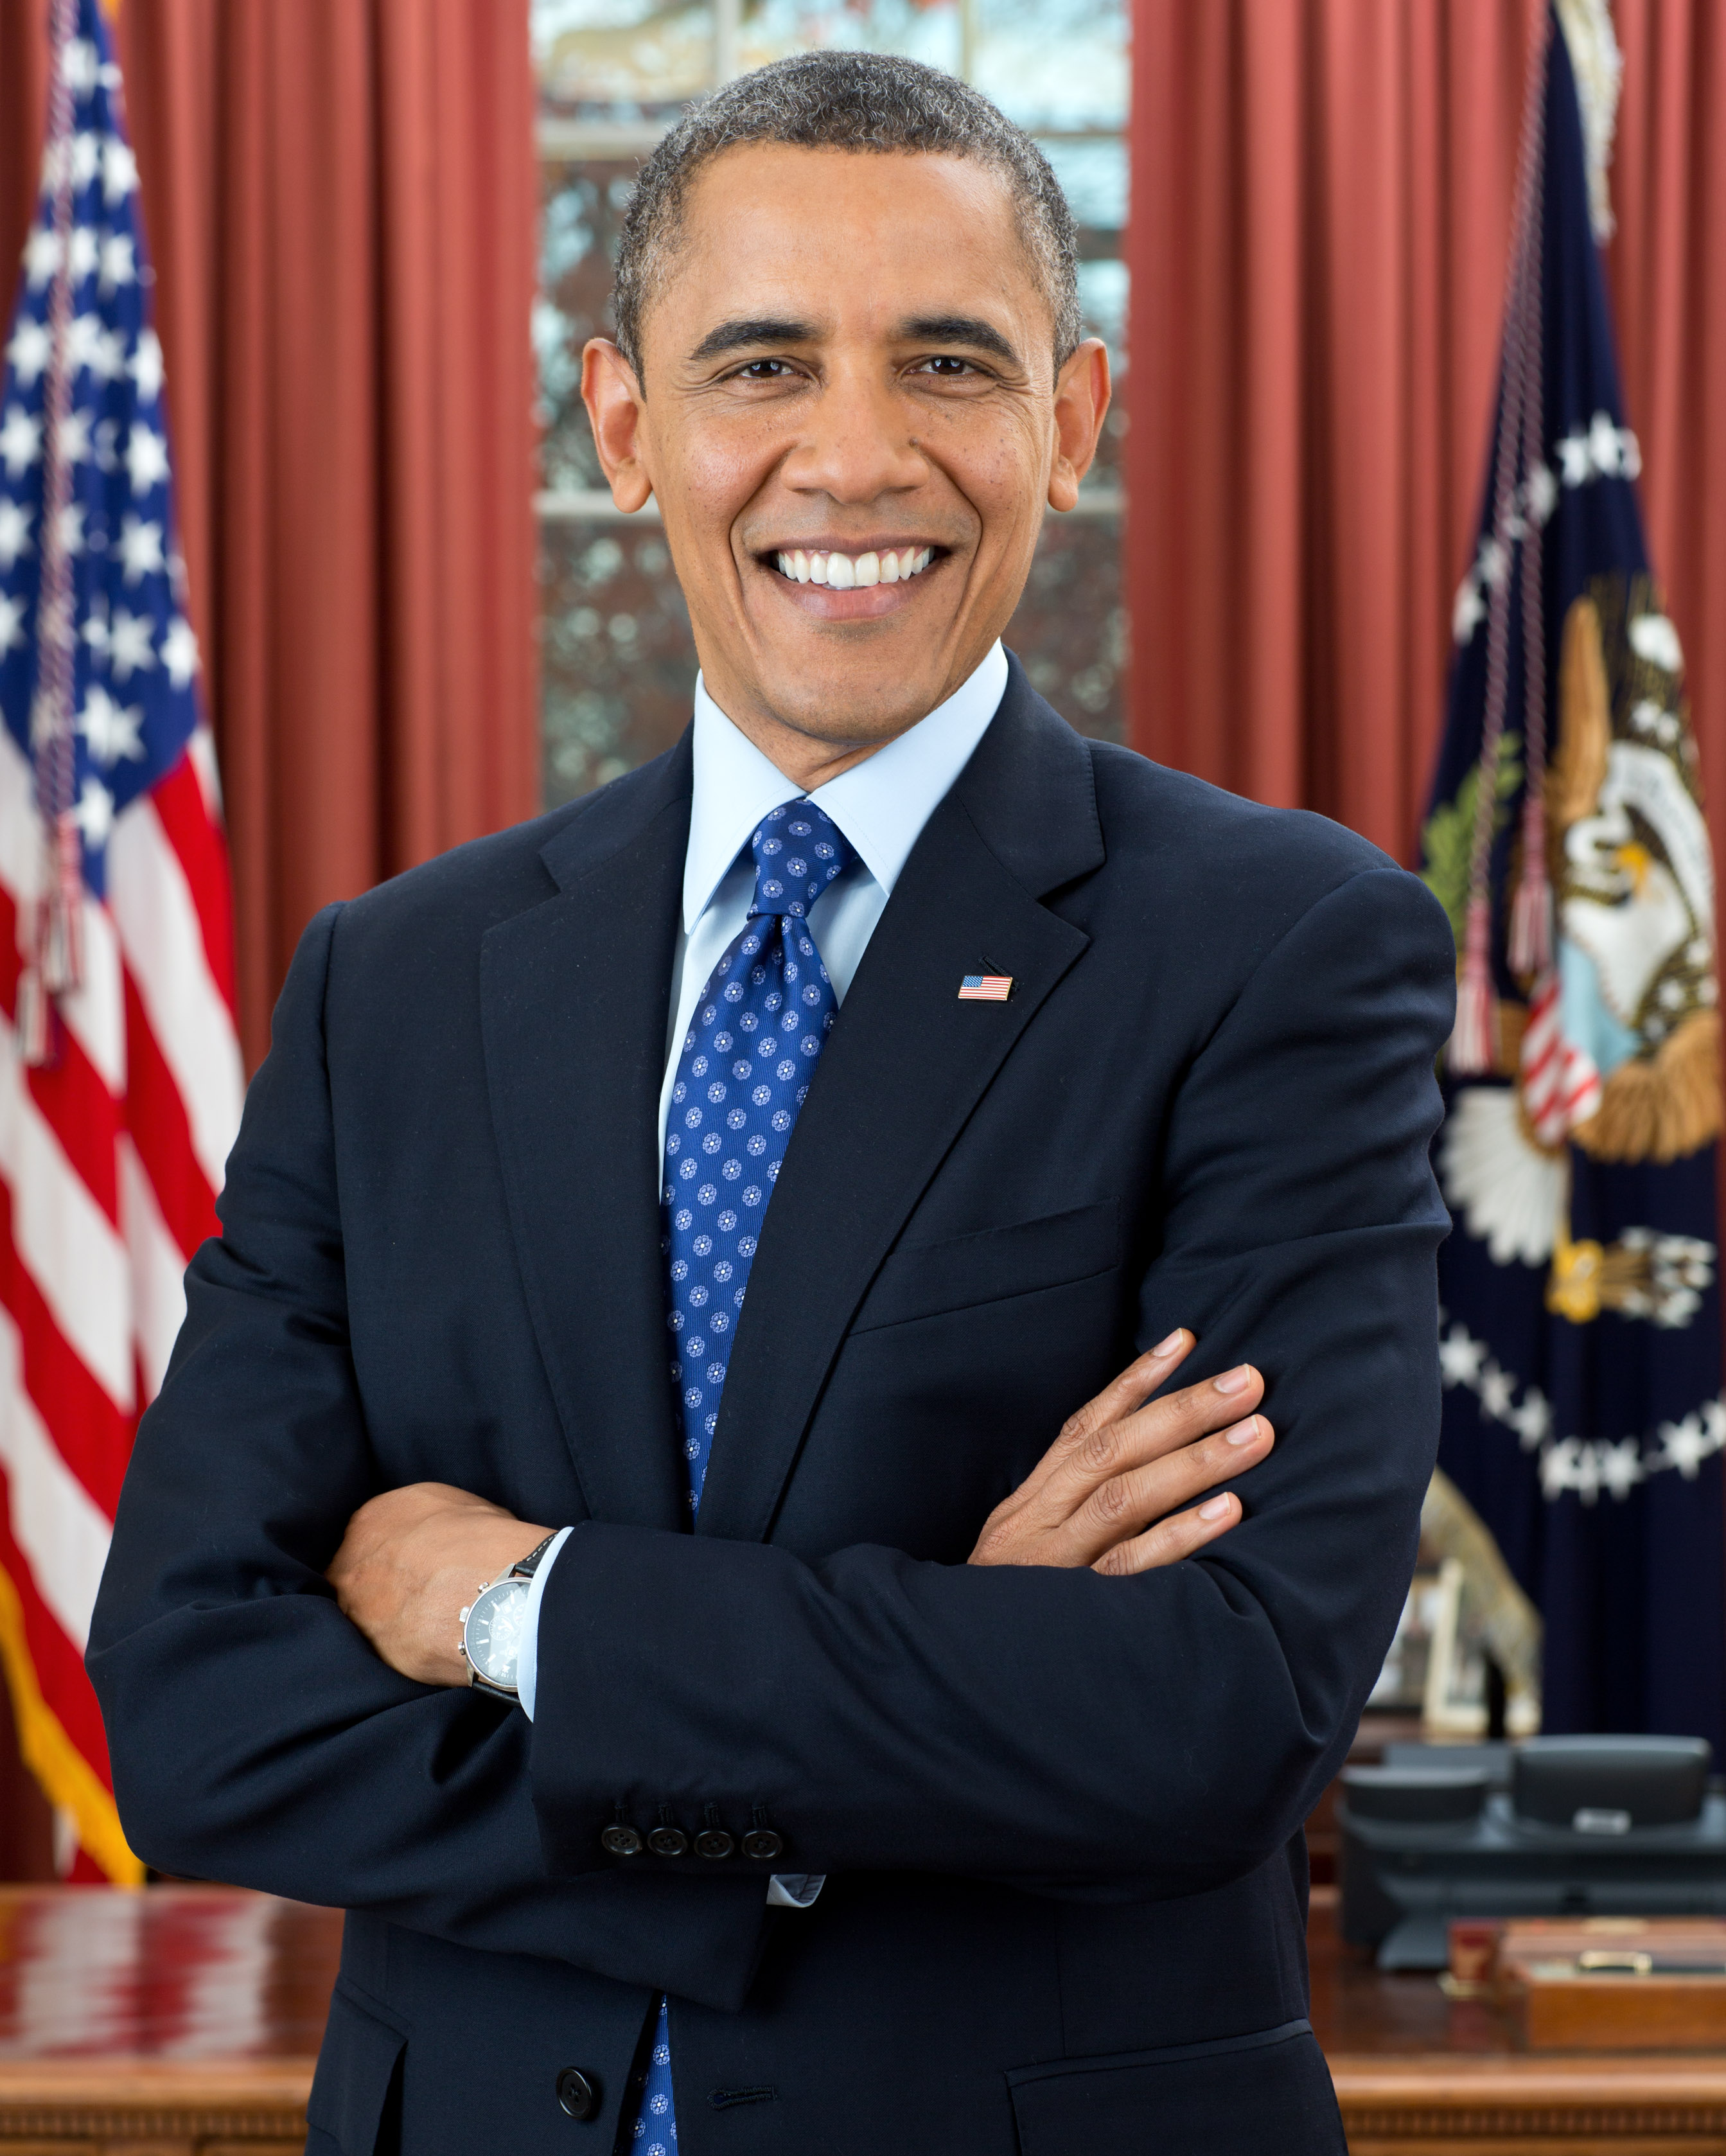
\includegraphics[width=0.5\textwidth,trim={0 9cm 0 0},clip]{figures/obama.jpg}\\
		\hspace*{15pt}\hbox{\scriptsize Image By:\thinspace{\itshape Pete Souza}}
		% https://commons.wikimedia.org/wiki/File:President_Barack_Obama.jpg
	\end{center}
\end{frame}

\begin{frame}
	\frametitle{An experiment!}
	
	\begin{itemize}
		\item We are going to perform a small demonstration of a first sorting algorithm.
			\pause
		\item It's called bubble sort, and as former president of the USA, Barack Obama, can tell you\dots
		\item You shouldn't want to use it: \url{https://www.youtu.be/koMpGeZpu4Q}
			\pause
		\item But it's a nice sorting idea I can show you in practice.
		\item We're with a pretty small group, so how about we do this all together? :)
	\end{itemize}
\end{frame}
